% CVPR 2027 review manuscript.
\documentclass[10pt,twocolumn,letterpaper]{article}
\usepackage[review]{cvpr}
\usepackage{amsmath,amssymb}
\usepackage{booktabs}
\usepackage{graphicx}
\usepackage{multirow}
\usepackage{tabularx}
\usepackage{xcolor}
\usepackage{microtype}
\usepackage{xspace}
\usepackage{enumitem}
\newcommand{\method}{PAIR-Audit\xspace}
\newcommand{\etal}{et al.\xspace}
\newcommand{\target}{\textsc{Target}\xspace}
\newcommand{\sham}{\textsc{Sham}\xspace}
\newcommand{\baseline}{\textsc{Baseline}\xspace}
\newcommand{\lfe}{LFE\xspace}
\newcommand{\R}{\mathbb{R}}
\setlength{\abovecaptionskip}{0.45em}
\setlength{\belowcaptionskip}{-0.25em}

\definecolor{cvprblue}{rgb}{0.21,0.49,0.74}
\usepackage[pagebackref,breaklinks,colorlinks,allcolors=cvprblue]{hyperref}
\def\confName{CVPR}
\def\confYear{2027}

\title{Readable Is Not Necessarily Causal:\\
A Preregistered Audit of Fine-Grained Identity Retention in Video Diffusion}

\author{Anonymous CVPR submission}

\begin{document}
\maketitle

\begin{abstract}
Identity-preserving video generators are commonly evaluated with global face similarity, although a reference identity can remain recognizable while local visible attributes drift.  Mechanistic analyses face a second gap: an attribute may be linearly readable from an internal representation, or covary with output retention, without that readout being a causal control variable.  We present \method, an auditable evidence ladder for separating output measurement, observational representation analysis, and paired intervention in a frozen reference-conditioned video diffusion transformer.  On ConsisID, we construct a fixed panel of 20 matched identity-attribute pairs spanning eyeglasses and facial hair.  Observational traces reveal heterogeneous attribute-direction signs across 32 local identity tokens, motivating—but not selecting—the intervention.  We then preregister a complete-family, leave-one-pair-out projection exchange at the Local Facial Extractor interface, with an equal-magnitude deterministic orthogonal sham.  A single transaction generates 480 trajectories (40 units, four seeds, three conditions), followed by condition-blind human annotation of 3,360 sampled frame states and complete adjudication.  The target-versus-sham effects are sparse and centered near zero: eyeglasses yields 0/7/3 correct/tie/wrong pairs (mean $-0.0232$), and facial hair yields 2/7/1 (mean $0.0051$).  Thus, under this fixed intervention and panel, readable directional structure does not provide broad, robust causal control of the generated attribute contrast.  The result constrains a simple linear mechanism; it does not imply that attribute information is absent from the local route.  We release the aggregate audit code, protocols, and cryptographic provenance while retaining identity-linked media privately.
\end{abstract}

\section{Introduction}
\label{sec:intro}

Diffusion transformers have made reference-conditioned human video generation increasingly realistic~\cite{ho2020ddpm,peebles2023dit,yang2024cogvideox}.  Identity-preserving systems inject face embeddings, reference features, or spatial image conditions to reduce identity drift~\cite{xu2024magicanimate,yuan2025consisid,cui2025hallo3,tu2025stableanimator,zhang2025magicmirror}.  Yet ``identity preservation'' is usually summarized by a global face-recognition score.  Such a score need not reveal whether a local, visually salient property—eyeglasses or facial hair, for example—survives generation.  Nor does an architecture diagram establish how the model uses attribute-related information.

Interpretability work on diffusion models increasingly discovers semantic directions, features, or layers and validates them through steering or ablation~\cite{li2024interpretdiffusion,dalva2024noiseclr,shi2025difflens,kulkarni2025posthoc,zaleska2026choices}.  This direction is promising, but it creates a demanding evidential question.  Linear readability is not causality; correlation with output behavior is not mediation; and an intervention can itself move a representation off the model's natural manifold~\cite{geiger2023causalabstraction,heimersheim2024patching,zhang2023patching,grant2025divergent}.  A convincing audit should therefore separate (i) what is visibly retained, (ii) what is observationally readable, and (iii) what changes under a matched, prospectively specified intervention.

We study this distinction in ConsisID~\cite{yuan2025consisid}, a tuning-free identity-preserving text-to-video system built on a diffusion-transformer backbone.  Its local identity route produces 32 Local Facial Extractor (LFE) tokens and injects them through 21 Perceiver cross-attention modules, while a separate spatial reference-latent route remains active.  This multi-route structure makes it a useful but difficult case: a direction can be present at the LFE interface without acting as an isolated causal bottleneck.

Figure~\ref{fig:overview} summarizes our evidence ladder.  We first establish attribute-specific output measurements on a frozen matched panel.  We then trace representation and injection summaries and conduct outcome-blind token-direction measurements.  These analyses motivate one narrow causal question: does exchanging the complete 32-token scalar projection along a leave-one-pair-out attribute direction change the generated positive-versus-control contrast relative to an equal-displacement orthogonal sham?  The target rule is complete-family and held-pair-out; no favorable token, pair, frame, or outcome selects the intervention.

\begin{figure*}[t]
  \centering
  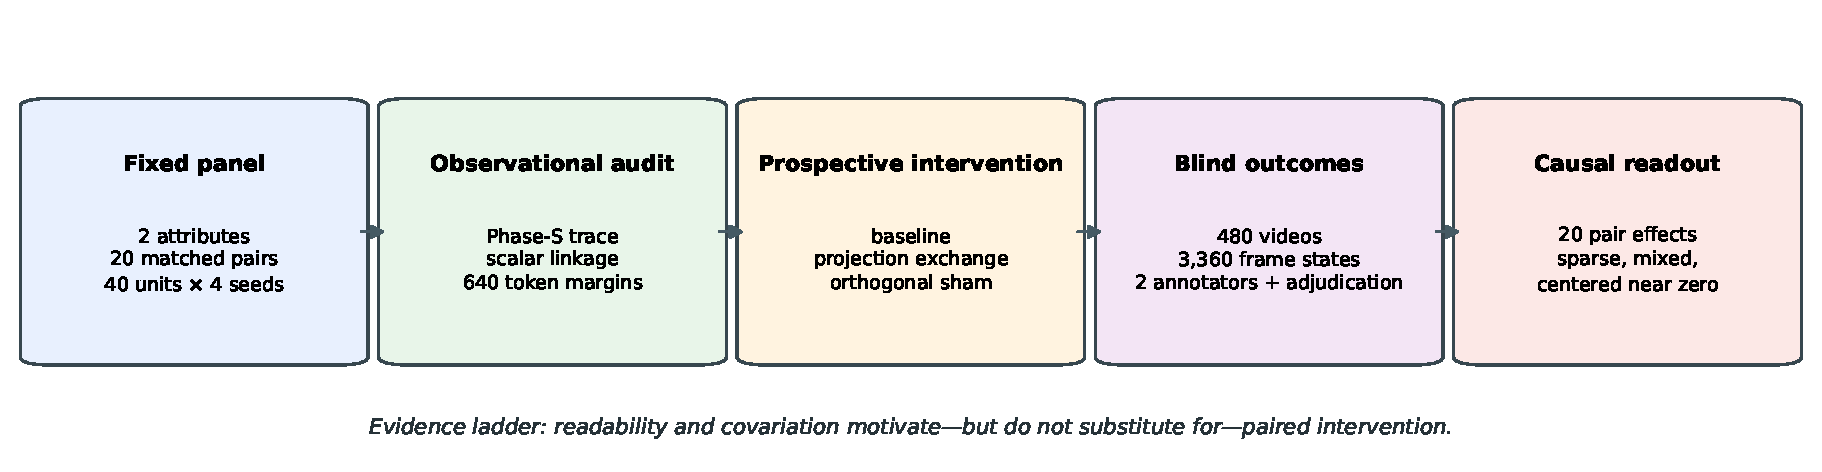
\includegraphics[width=\textwidth]{figures/audit_overview.pdf}
  \caption{\textbf{Auditable evidence ladder.}  Output measurement and observational internal analyses motivate a prospectively frozen projection-exchange intervention; they are not treated as causal evidence.  Only aggregate, identity-disconnected artifacts are used in the paper.}
  \label{fig:overview}
\end{figure*}

Our contributions are:
\begin{itemize}[leftmargin=*,nosep]
  \item an auditable protocol that separates fine-grained output measurement, observational representation analysis, and paired causal intervention in reference-conditioned video diffusion;
  \item a complete-family intervention that exchanges leave-one-pair-out LFE projections and compares them with a deterministic orthogonal sham of identical per-token displacement magnitude;
  \item a preregistered 480-trajectory experiment with two independent blinded annotations, complete disagreement adjudication, no reduced panel, and independently verified persisted artifacts; and
  \item evidence that observational directional readability does not translate into a broad, robust target-specific effect in this fixed setting, while preserving the narrower claim boundary that LFE information absence and route irrelevance are not established.
\end{itemize}

\section{Related Work}
\label{sec:related}

\paragraph{Identity-preserving video generation.}
Human image animation and personalized video diffusion use appearance encoders, face features, reference networks, or specialized training to preserve identity~\cite{xu2024magicanimate,cui2025hallo3,tu2025stableanimator,zhang2025magicmirror}.  ConsisID decomposes identity conditioning into frequency-motivated local and global signals~\cite{yuan2025consisid}; more recent systems optimize identity rewards~\cite{shen2026ipro} or add multi-view appearance and geometry~\cite{wu2026considgen}.  These works primarily improve generation quality.  We instead audit one frozen model and ask whether a particular internal attribute direction contributes causally to fine-grained retention.  Our goal is neither a new generator nor a cross-model benchmark.

\paragraph{Interpretable directions in generative models.}
Latent directions and concept controllers can expose and manipulate semantic factors in diffusion models~\cite{li2024interpretdiffusion,dalva2024noiseclr,kulkarni2025posthoc}.  DiffLens identifies and intervenes on internal features associated with biased generation~\cite{shi2025difflens}; layer-localization and causal suppression studies further show that apparent salience and functional importance can diverge~\cite{zaleska2026choices,wu2026attentionsinks}.  Our study complements successful steering results with a complete, prospectively specified negative/mixed intervention result.  The scientific object is the boundary between a readable direction and a robust causal control variable.

\paragraph{Interchange interventions and causal claims.}
Activation patching and interchange interventions compare counterfactual internal states, but their conclusions depend on the patched variable, corruption/intervention rule, metric, and distribution shift~\cite{heimersheim2024patching,zhang2023patching}.  Causal abstraction formalizes when low-level interventions can realize higher-level variables~\cite{geiger2023causalabstraction,geiger2024das}.  We adopt the operational discipline—not the claim that a full abstraction has been found—by specifying a held-out direction, a matched sham, a fixed outcome, and explicit non-claims.

\section{System and Fixed Panel}
\label{sec:setup}

\subsection{Two reference-conditioning routes}

We audit the public ConsisID implementation at a frozen source revision.  The local route combines an InsightFace-style 512-D face embedding~\cite{deng2019arcface}, a normalized 768-D EVA output, and five EVA hidden-state maps.  The LFE maps these inputs to
\begin{equation}
  X_u \in \R^{32\times 2048},
\end{equation}
for reference unit $u$.  Twenty-one distinct Perceiver cross-attention modules inject these tokens as keys/values after transformer blocks $0,2,\ldots,40$; video tokens supply the queries.  The same route is available at all 50 scheduler positions.

A separate spatial route VAE-encodes the aligned reference face into the first reference-latent frame and pads later reference frames with zeros before concatenation with the noisy video latent.  The local intervention in Sec.~\ref{sec:intervention} leaves this spatial route, text conditioning, global identity inputs, scheduler, and weights unchanged.  There is no attribute-specific mask in either the LFE or its injection modules.

\subsection{Frozen matched panel and generation settings}

The formal panel contains two visible attributes—eyeglasses and facial hair—with ten frozen matched positive/control pairs per attribute.  This gives 40 reference units.  Each unit has four fixed seeds, producing 160 source tasks.  Reference, prompt, negative prompt, scheduler, guidance ($6.0$), precision (bfloat16), resolution ($480\times720$), 49 decoded frames, and all exclusion rules are fixed.  Pairs, not frames, are the scientific units for the final intervention summary.

The original output-measurement panel generated one video per unit/seed.  Eyeglasses uses frozen human consensus as the primary measurement; a detector-plus-CLIP pipeline~\cite{radford2021clip} is retained only as secondary convergence evidence.  Facial hair uses a frozen human ordinal rubric.  In the original panel, the 40 eyeglasses seed-pair differences were 33 positive, seven zero, and zero negative (mean $0.825$); facial-hair pair differences were heterogeneous (mean $0.205$, median $0$, range $[-1,1]$).  These observations establish that the attributes are measurable in the panel, not why retention succeeds or fails.

\section{From Readability to a Causal Test}
\label{sec:observational}

\subsection{Observational evidence ladder}

We summarize earlier closed analysis windows because they motivate the intervention but do not enter its parameter selection (Table~\ref{tab:ladder}).  A bounded Phase-S transaction traced all 160 tasks and 8,000 transformer steps.  The pooled LFE margin had 5/0/5 correct/tie/wrong pairs for eyeglasses and 6/0/4 for facial hair; all 36 injection-grid cells contained both pair-difference signs.  Fixed-panel Spearman linkage between pooled LFE margins and output contrasts was $0.121$ for eyeglasses and $0.494$ for facial hair.  These are descriptive coefficients over ten pairs, without population or mediation interpretation.

An outcome-blind token-direction transaction then recomputed the complete 32-token family.  Across 320 pair-token margins per attribute, eyeglasses had 145 positive and 175 negative signs; facial hair had 173 positive and 147 negative signs.  All pairs contained both signs across tokens, and 29/32 eyeglasses token indices and 32/32 facial-hair indices were mixed across pairs.  Within the current transaction, direct-repeat controls were bit-exact.  Relative to historical Phase-S summaries, strict numerical matches were 0/20 while signs matched 20/20, so the historical numerical mismatch is retained rather than repaired.

\begin{table}[t]
\centering
\caption{Closed evidence windows.  Each row has a deliberately bounded inference.}
\label{tab:ladder}
\resizebox{\columnwidth}{!}{%
\begin{tabular}{@{}lll@{}}
\toprule
Stage & Main observation & Allowed inference \\
\midrule
Output panel & Attribute contrasts visible & Fixed-panel retention \\
Phase-S trace & Mixed LFE/injection signs & Readability is heterogeneous \\
Scalar linkage & $\rho=0.121/0.494$ & Descriptive covariation \\
Token direction & 640 mixed margins & Pair/token dependence \\
Intervention & 20 target--sham effects & Effect of fixed manipulation \\
\bottomrule
\end{tabular}}
\end{table}

These results rule out selecting a single ``best'' token from the observed family.  They motivate a complete-family test: intervene on every token with directions rebuilt from the current acquisition transaction, while holding each evaluated pair out.

\subsection{Preregistered intervention question}

For attribute $a$, held pair $p$, and token $k$, let $X_{u,k}\in\R^{2048}$ be the transient LFE token for unit $u$, and
\begin{equation}
 Z_{u,k}=\frac{X_{u,k}}{\max(\lVert X_{u,k}\rVert_2,10^{-12})}.
\end{equation}
Using the other nine pairs of the same attribute, we define
\begin{align}
 d_{a,p,k} &= \frac{1}{9}\sum_{q\ne p}\left(Z_{\mathrm{pos}(q),k}-Z_{\mathrm{ctrl}(q),k}\right),\\
 u_{a,p,k} &= d_{a,p,k}/\lVert d_{a,p,k}\rVert_2.
\end{align}
Every evaluated pair is therefore out-of-sample with respect to its direction.  All 32 token directions are used; no observational margin or outcome selects or weights them.

\section{Matched Projection Exchange}
\label{sec:intervention}

\subsection{Target and orthogonal-sham conditions}

For role $r\in\{\mathrm{pos},\mathrm{ctrl}\}$ and its counterpart $\bar r$, define the scalar displacement
\begin{equation}
 \delta_{r,k}=\left\langle X_{\bar r,k}-X_{r,k},u_{a,p,k}\right\rangle.
\end{equation}
The \target condition exactly exchanges the two units' raw scalar projections along the held-pair-out direction:
\begin{equation}
 X^{\mathrm{target}}_{r,k}=X_{r,k}+\delta_{r,k}u_{a,p,k}.
\end{equation}

For the \sham condition, a deterministic SHAKE256-seeded Rademacher vector is orthogonalized against $u_{a,p,k}$ and normalized to $q_{a,p,k}$.  We set
\begin{equation}
 X^{\mathrm{sham}}_{r,k}=X_{r,k}+\delta_{r,k}q_{a,p,k},\qquad
 \langle q,u\rangle=0.
\end{equation}
Thus target and sham have equal per-token displacement norm, while the sham preserves the original target-direction projection.  This controls displacement magnitude, not all off-manifold or downstream consequences.  The \baseline condition leaves $X$ unchanged.

The selected LFE tensor replaces the normal tensor at all 21 injection sites, all 50 scheduler positions, and every classifier-free-guidance row.  All conditions for a task restart from the same seed and initial latent with a fresh scheduler.  Condition order is deterministically permuted from the task identifier before model loading.

\subsection{Acquisition and execution invariants}

One loaded process performs exactly 40 fresh preprocessing calls and 40 direct LFE acquisitions in ascending unit order before any trajectory.  Tensors remain in memory and are shared across the four seeds and three conditions of each unit; no raw identity or LFE tensor is persisted.  Before generation, one-step controls verify the baseline hook against the cached direct tensor.  All 640 directions are finite and unit-norm; target counterpart projections match; sham displacements are orthogonal; and target/sham norms match at frozen tolerances.  A failure aborts the transaction rather than dropping a token, pair, task, or condition.

The scientific transaction completes all $40\times4\times3=480$ trajectories and 24,000 scheduler steps on one GPU in 35.56 GPU-hours.  It persists 480 private final latents but no raw LFE/direction tensor and no decoded media during generation.  A separately authorized private decode produces 480 videos and 23,520 frames in 0.74 GPU-hours; all source latents and decoded artifacts pass independent byte/hash and media-contract verification.

\subsection{Blind outcome construction}

For each video, only frames $\{0,8,16,24,32,40,48\}$ are sampled, giving 3,360 frame states.  Two annotators receive pseudonymous, condition-blind items mixing attributes, pairs, roles, conditions, and seeds.  Eyeglasses labels are \texttt{present}, \texttt{absent}, or unobservable (U).  Facial-hair labels are ordinal $0/1/2/$U; the preregistered primary score maps $1$ and $2$ to present.  Annotators agree directly on 1,521 states; all 1,839 disagreements are adjudicated before unblinding.  Independence is researcher-attested rather than inferable from the submitted CSVs.

Each unit-condition score $S_{r,c}$ is the present fraction among valid labels pooled over four seeds and seven frames (28 planned states); U states remain missing rather than being imputed.  All 120 unit-condition scores are defined.

\subsection{Primary estimand}

For role $r$, let $C_r=S_{r,\mathrm{target}}-S_{r,\mathrm{sham}}$.  Because projection exchange is predicted to increase the attribute for the control role and decrease it for the positive role, the pair effect is
\begin{equation}
 E_{a,p}=\tfrac{1}{2}\left(C_{\mathrm{ctrl}}-C_{\mathrm{pos}}\right).
 \label{eq:estimand}
\end{equation}
A positive value is the preregistered direction; $|E|\le10^{-8}$ is a tie.  We report all ten values per attribute plus correct/tie/wrong counts, mean, median, and range.  The design intentionally specifies no $p$-value, confidence interval, cross-attribute pooling, or reduced-panel aggregate.

\section{Results}
\label{sec:results}

\subsection{Coverage and completion}

No pair effect is missing and no frame, pair, seed, or trajectory is regenerated or excluded.  Eyeglasses valid-state coverage is 530/560 for baseline, 531/560 for target, and 533/560 for sham.  Facial-hair coverage is respectively 379/560, 382/560, and 380/560.  The 625 U states and their reasons are retained in the authoritative corrected unblinding record.  These rates show that facial hair is substantially less observable, but every unit-condition still has at least one valid state.

\subsection{Primary target-versus-sham effects}

Table~\ref{tab:primary} and Fig.~\ref{fig:effects} give the complete primary family.  Eyeglasses has no positive pair effect: seven ties and three effects in the wrong direction.  The mean is $-0.0232$, median $0$, and range $[-0.125,0]$.  Facial hair has two positive effects (FFH\_08 and FFH\_09), seven ties, and one wrong-direction effect (FFH\_10).  Its mean is $0.0051$, median $0$, and range $[-0.0292,0.0556]$.

\begin{table}[t]
\centering
\caption{Complete preregistered primary results.  C/T/W denotes correct/tie/wrong relative to the predicted positive direction.}
\label{tab:primary}
\resizebox{\columnwidth}{!}{%
\begin{tabular}{@{}lrrrrr@{}}
\toprule
Attribute & Pairs & C/T/W & Mean & Median & Range \\
\midrule
Eyeglasses & 10 & 0/7/3 & $-0.0232$ & 0 & $[-0.125,0]$ \\
Facial hair & 10 & 2/7/1 & $0.0051$ & 0 & $[-0.0292,0.0556]$ \\
\bottomrule
\end{tabular}}
\end{table}

\begin{figure*}[t]
  \centering
  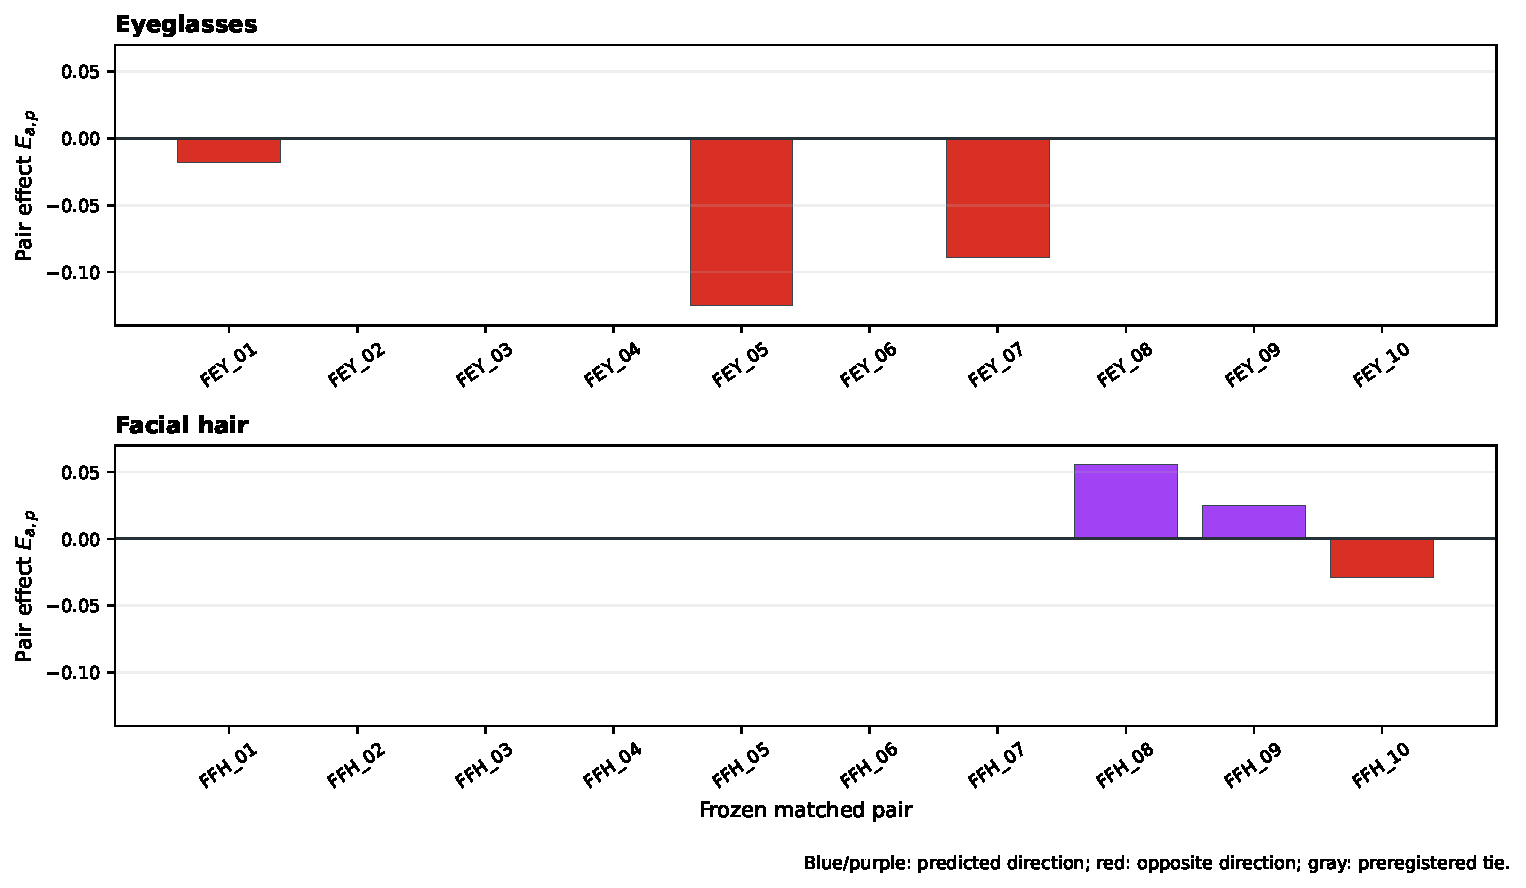
\includegraphics[width=0.94\textwidth]{figures/pair_effects.pdf}
  \caption{\textbf{All 20 preregistered pair effects.}  Positive values follow the predicted target direction, red values are opposite, and zero values are ties.  The family is sparse and mixed rather than predominantly positive.}
  \label{fig:effects}
\end{figure*}

The complete secondary contrasts do not support a generic target-specific rescue.  For FEY\_01, the role-aligned sham-minus-baseline effect ($0.125$) exceeds target-minus-baseline ($0.107$), producing a negative target-versus-sham effect.  FEY\_05 and FEY\_07 move in the wrong target direction while sham is unchanged.  For facial hair, FFH\_08 and FFH\_09 move modestly in the predicted direction; FFH\_10 moves oppositely, and FFH\_04 shows the same small target and sham movement relative to baseline.

\subsection{What the intervention changes scientifically}

The observational analyses established heterogeneous readable structure but could not distinguish a causal variable from a correlated readout.  The complete intervention supplies that missing test for one operational hypothesis.  Under the fixed dose, complete token family, LFE interface, and finite panel, exchanging the held-pair-out scalar projection does \emph{not} yield a broad, robust direction-specific change relative to equal-magnitude orthogonal displacement.  Limited pair-specific facial-hair evidence remains visible, but it coexists with a counterexample and does not generalize to eyeglasses.

\section{Discussion}
\label{sec:discussion}

\paragraph{Readable is not necessarily causal.}
The central result is a separation between observational readability and causal manipulability.  Phase-S, scalar linkage, and token directions all reveal nontrivial internal structure.  Nevertheless, a prospectively frozen intervention on that structure produces mostly ties, four wrong-direction effects, and only two modest positive effects.  This does not make the observational results erroneous; it limits the interpretation that may be attached to them.

\paragraph{What the result rules out.}
The data do not support a simple claim that the complete held-pair-out linear projection is a broad causal controller of the positive-versus-control output contrast.  This conclusion is stronger than a failed post-hoc steering attempt because the target family, dose, sham, task universe, outcome, and failure policy were fixed before outcome access, and every pair is retained.

\paragraph{What the result does not rule out.}
The experiment does not establish that LFE lacks attribute information or that the local route is irrelevant.  At least four alternatives remain: (i) downstream use is nonlinear or query/state dependent; (ii) the projection exchange is partly off-manifold; (iii) the independently active spatial route compensates or interacts; and (iv) the frozen human score has limited sensitivity near floors or ceilings.  The accepted working model—representation/readout mismatch or reorganization in a multi-path distributed system—is compatible with the evidence, but is not itself verified.

\paragraph{Measurement state.}
Many unit-condition scores are saturated: all eyeglasses control scores are zero, and many positive-role scores are one.  Facial-hair positives are also often one.  Saturation restricts detectable movement.  We retain it as a limitation rather than changing the metric after observing results.  Likewise, the large adjudicated subset indicates perceptual ambiguity even though the final outcome table is complete.

\paragraph{Why the sham matters.}
An orthogonal equal-displacement sham is not a perfect null—it may still perturb the model off-manifold—but it prevents any observed change from being attributed merely to displacement magnitude.  FEY\_01 and FFH\_04 illustrate why baseline alone would overstate direction specificity: generic perturbation can match or exceed the target change.

\section{Limitations and Scope}
\label{sec:limitations}

This is a single-model, single-checkpoint study with two attributes and ten pairs per attribute.  It is not a population estimate and cannot rank inherent attribute difficulty.  The primary family is descriptive by preregistration; the study provides no confidence intervals or significance tests.  Four seeds reduce trajectory noise within each unit but do not create 40 independent pair observations.  Human annotations are complete after adjudication, yet annotator independence is an attestation and direct agreement is limited.  The intervention is linear and fixed-dose, and the sham controls magnitude rather than manifold membership.  We do not separate the local and spatial routes, identify a bottleneck, or establish natural mediation, necessity, sufficiency, localization, frame independence, or model-wide behavior.  Finally, privacy constraints prevent release of reference-linked videos and qualitative identity panels; reproducibility therefore relies on code, aggregate tables, protocols, hashes, and independent verification rather than public media.

\section{Ethics, Privacy, and Reproducibility}
\label{sec:ethics}

Identity-conditioned generation can facilitate impersonation and can expose biometric or appearance information.  We therefore retain reference images, identity names, aligned faces, embeddings, LFE tensors, private latents, decoded videos, annotation frames, and blind mappings outside the public repository.  The paper reports only aggregate, pseudonymous results.  No fine-tuning or LoRA is performed and no reference-corresponding generated video is released.  This restriction reduces qualitative reproducibility but limits privacy and misuse risk.

The audit is append-only and fail-closed.  Frozen CSV/JSON artifacts bind inputs and outputs by byte count and SHA256; historical failures are preserved rather than overwritten; runtime directories are read-only; and independent verifiers recompute enumeration, invariants, hashes, outcomes, and pair effects.  Source code and aggregate artifacts will be made available in an anonymized supplement subject to venue policy.

\section{Conclusion}

We presented an evidence ladder for fine-grained identity retention that distinguishes visible output, observational internal structure, and causal intervention.  In a complete, preregistered ConsisID transaction, leave-one-pair-out LFE projection exchange does not produce a predominant target-specific effect over a matched orthogonal sham.  The result is best understood as a mechanism constraint: a readable linear direction is not, by itself, a robust causal control variable.  Stronger claims about information absence, route irrelevance, compensation, or distributed mechanisms require distinct prospective experiments.

{\small
\bibliographystyle{ieeenat_fullname}
\bibliography{references}
}

\section*{LLM Usage Statement}
An OpenAI language model was used to assist with literature discovery, manuscript drafting and language editing, and code generation for presentation-only figures.  The authors remain responsible for the manuscript and independently verified all numerical values and scientific claims against frozen artifacts, and all citations against primary sources.  No language model generated experimental labels, outcomes, interventions, or scientific results.

\end{document}
